% Options for packages loaded elsewhere
\PassOptionsToPackage{unicode}{hyperref}
\PassOptionsToPackage{hyphens}{url}
\PassOptionsToPackage{dvipsnames,svgnames,x11names}{xcolor}
%
\documentclass[
  letterpaper,
  DIV=11,
  numbers=noendperiod]{scrartcl}

\usepackage{amsmath,amssymb}
\usepackage{lmodern}
\usepackage{iftex}
\ifPDFTeX
  \usepackage[T1]{fontenc}
  \usepackage[utf8]{inputenc}
  \usepackage{textcomp} % provide euro and other symbols
\else % if luatex or xetex
  \usepackage{unicode-math}
  \defaultfontfeatures{Scale=MatchLowercase}
  \defaultfontfeatures[\rmfamily]{Ligatures=TeX,Scale=1}
\fi
% Use upquote if available, for straight quotes in verbatim environments
\IfFileExists{upquote.sty}{\usepackage{upquote}}{}
\IfFileExists{microtype.sty}{% use microtype if available
  \usepackage[]{microtype}
  \UseMicrotypeSet[protrusion]{basicmath} % disable protrusion for tt fonts
}{}
\makeatletter
\@ifundefined{KOMAClassName}{% if non-KOMA class
  \IfFileExists{parskip.sty}{%
    \usepackage{parskip}
  }{% else
    \setlength{\parindent}{0pt}
    \setlength{\parskip}{6pt plus 2pt minus 1pt}}
}{% if KOMA class
  \KOMAoptions{parskip=half}}
\makeatother
\usepackage{xcolor}
\setlength{\emergencystretch}{3em} % prevent overfull lines
\setcounter{secnumdepth}{-\maxdimen} % remove section numbering
% Make \paragraph and \subparagraph free-standing
\ifx\paragraph\undefined\else
  \let\oldparagraph\paragraph
  \renewcommand{\paragraph}[1]{\oldparagraph{#1}\mbox{}}
\fi
\ifx\subparagraph\undefined\else
  \let\oldsubparagraph\subparagraph
  \renewcommand{\subparagraph}[1]{\oldsubparagraph{#1}\mbox{}}
\fi

\usepackage{color}
\usepackage{fancyvrb}
\newcommand{\VerbBar}{|}
\newcommand{\VERB}{\Verb[commandchars=\\\{\}]}
\DefineVerbatimEnvironment{Highlighting}{Verbatim}{commandchars=\\\{\}}
% Add ',fontsize=\small' for more characters per line
\usepackage{framed}
\definecolor{shadecolor}{RGB}{241,243,245}
\newenvironment{Shaded}{\begin{snugshade}}{\end{snugshade}}
\newcommand{\AlertTok}[1]{\textcolor[rgb]{0.68,0.00,0.00}{#1}}
\newcommand{\AnnotationTok}[1]{\textcolor[rgb]{0.37,0.37,0.37}{#1}}
\newcommand{\AttributeTok}[1]{\textcolor[rgb]{0.40,0.45,0.13}{#1}}
\newcommand{\BaseNTok}[1]{\textcolor[rgb]{0.68,0.00,0.00}{#1}}
\newcommand{\BuiltInTok}[1]{\textcolor[rgb]{0.00,0.23,0.31}{#1}}
\newcommand{\CharTok}[1]{\textcolor[rgb]{0.13,0.47,0.30}{#1}}
\newcommand{\CommentTok}[1]{\textcolor[rgb]{0.37,0.37,0.37}{#1}}
\newcommand{\CommentVarTok}[1]{\textcolor[rgb]{0.37,0.37,0.37}{\textit{#1}}}
\newcommand{\ConstantTok}[1]{\textcolor[rgb]{0.56,0.35,0.01}{#1}}
\newcommand{\ControlFlowTok}[1]{\textcolor[rgb]{0.00,0.23,0.31}{#1}}
\newcommand{\DataTypeTok}[1]{\textcolor[rgb]{0.68,0.00,0.00}{#1}}
\newcommand{\DecValTok}[1]{\textcolor[rgb]{0.68,0.00,0.00}{#1}}
\newcommand{\DocumentationTok}[1]{\textcolor[rgb]{0.37,0.37,0.37}{\textit{#1}}}
\newcommand{\ErrorTok}[1]{\textcolor[rgb]{0.68,0.00,0.00}{#1}}
\newcommand{\ExtensionTok}[1]{\textcolor[rgb]{0.00,0.23,0.31}{#1}}
\newcommand{\FloatTok}[1]{\textcolor[rgb]{0.68,0.00,0.00}{#1}}
\newcommand{\FunctionTok}[1]{\textcolor[rgb]{0.28,0.35,0.67}{#1}}
\newcommand{\ImportTok}[1]{\textcolor[rgb]{0.00,0.46,0.62}{#1}}
\newcommand{\InformationTok}[1]{\textcolor[rgb]{0.37,0.37,0.37}{#1}}
\newcommand{\KeywordTok}[1]{\textcolor[rgb]{0.00,0.23,0.31}{#1}}
\newcommand{\NormalTok}[1]{\textcolor[rgb]{0.00,0.23,0.31}{#1}}
\newcommand{\OperatorTok}[1]{\textcolor[rgb]{0.37,0.37,0.37}{#1}}
\newcommand{\OtherTok}[1]{\textcolor[rgb]{0.00,0.23,0.31}{#1}}
\newcommand{\PreprocessorTok}[1]{\textcolor[rgb]{0.68,0.00,0.00}{#1}}
\newcommand{\RegionMarkerTok}[1]{\textcolor[rgb]{0.00,0.23,0.31}{#1}}
\newcommand{\SpecialCharTok}[1]{\textcolor[rgb]{0.37,0.37,0.37}{#1}}
\newcommand{\SpecialStringTok}[1]{\textcolor[rgb]{0.13,0.47,0.30}{#1}}
\newcommand{\StringTok}[1]{\textcolor[rgb]{0.13,0.47,0.30}{#1}}
\newcommand{\VariableTok}[1]{\textcolor[rgb]{0.07,0.07,0.07}{#1}}
\newcommand{\VerbatimStringTok}[1]{\textcolor[rgb]{0.13,0.47,0.30}{#1}}
\newcommand{\WarningTok}[1]{\textcolor[rgb]{0.37,0.37,0.37}{\textit{#1}}}

\providecommand{\tightlist}{%
  \setlength{\itemsep}{0pt}\setlength{\parskip}{0pt}}\usepackage{longtable,booktabs,array}
\usepackage{calc} % for calculating minipage widths
% Correct order of tables after \paragraph or \subparagraph
\usepackage{etoolbox}
\makeatletter
\patchcmd\longtable{\par}{\if@noskipsec\mbox{}\fi\par}{}{}
\makeatother
% Allow footnotes in longtable head/foot
\IfFileExists{footnotehyper.sty}{\usepackage{footnotehyper}}{\usepackage{footnote}}
\makesavenoteenv{longtable}
\usepackage{graphicx}
\makeatletter
\def\maxwidth{\ifdim\Gin@nat@width>\linewidth\linewidth\else\Gin@nat@width\fi}
\def\maxheight{\ifdim\Gin@nat@height>\textheight\textheight\else\Gin@nat@height\fi}
\makeatother
% Scale images if necessary, so that they will not overflow the page
% margins by default, and it is still possible to overwrite the defaults
% using explicit options in \includegraphics[width, height, ...]{}
\setkeys{Gin}{width=\maxwidth,height=\maxheight,keepaspectratio}
% Set default figure placement to htbp
\makeatletter
\def\fps@figure{htbp}
\makeatother
\newlength{\cslhangindent}
\setlength{\cslhangindent}{1.5em}
\newlength{\csllabelwidth}
\setlength{\csllabelwidth}{3em}
\newlength{\cslentryspacingunit} % times entry-spacing
\setlength{\cslentryspacingunit}{\parskip}
\newenvironment{CSLReferences}[2] % #1 hanging-ident, #2 entry spacing
 {% don't indent paragraphs
  \setlength{\parindent}{0pt}
  % turn on hanging indent if param 1 is 1
  \ifodd #1
  \let\oldpar\par
  \def\par{\hangindent=\cslhangindent\oldpar}
  \fi
  % set entry spacing
  \setlength{\parskip}{#2\cslentryspacingunit}
 }%
 {}
\usepackage{calc}
\newcommand{\CSLBlock}[1]{#1\hfill\break}
\newcommand{\CSLLeftMargin}[1]{\parbox[t]{\csllabelwidth}{#1}}
\newcommand{\CSLRightInline}[1]{\parbox[t]{\linewidth - \csllabelwidth}{#1}\break}
\newcommand{\CSLIndent}[1]{\hspace{\cslhangindent}#1}

\KOMAoption{captions}{tableheading}
\makeatletter
\makeatother
\makeatletter
\makeatother
\makeatletter
\@ifpackageloaded{caption}{}{\usepackage{caption}}
\AtBeginDocument{%
\ifdefined\contentsname
  \renewcommand*\contentsname{Table of contents}
\else
  \newcommand\contentsname{Table of contents}
\fi
\ifdefined\listfigurename
  \renewcommand*\listfigurename{List of Figures}
\else
  \newcommand\listfigurename{List of Figures}
\fi
\ifdefined\listtablename
  \renewcommand*\listtablename{List of Tables}
\else
  \newcommand\listtablename{List of Tables}
\fi
\ifdefined\figurename
  \renewcommand*\figurename{Figure}
\else
  \newcommand\figurename{Figure}
\fi
\ifdefined\tablename
  \renewcommand*\tablename{Table}
\else
  \newcommand\tablename{Table}
\fi
}
\@ifpackageloaded{float}{}{\usepackage{float}}
\floatstyle{ruled}
\@ifundefined{c@chapter}{\newfloat{codelisting}{h}{lop}}{\newfloat{codelisting}{h}{lop}[chapter]}
\floatname{codelisting}{Listing}
\newcommand*\listoflistings{\listof{codelisting}{List of Listings}}
\makeatother
\makeatletter
\@ifpackageloaded{caption}{}{\usepackage{caption}}
\@ifpackageloaded{subcaption}{}{\usepackage{subcaption}}
\makeatother
\makeatletter
\@ifpackageloaded{tcolorbox}{}{\usepackage[many]{tcolorbox}}
\makeatother
\makeatletter
\@ifundefined{shadecolor}{\definecolor{shadecolor}{rgb}{.97, .97, .97}}
\makeatother
\makeatletter
\makeatother
\ifLuaTeX
  \usepackage{selnolig}  % disable illegal ligatures
\fi
\IfFileExists{bookmark.sty}{\usepackage{bookmark}}{\usepackage{hyperref}}
\IfFileExists{xurl.sty}{\usepackage{xurl}}{} % add URL line breaks if available
\urlstyle{same} % disable monospaced font for URLs
\hypersetup{
  pdftitle={IMRaD report for Karl},
  pdfauthor={Alexandra Stephenson},
  colorlinks=true,
  linkcolor={blue},
  filecolor={Maroon},
  citecolor={Blue},
  urlcolor={Blue},
  pdfcreator={LaTeX via pandoc}}

\title{IMRaD report for Karl}
\author{Alexandra Stephenson}
\date{5/24/23}

\begin{document}
\maketitle
\ifdefined\Shaded\renewenvironment{Shaded}{\begin{tcolorbox}[frame hidden, sharp corners, enhanced, interior hidden, boxrule=0pt, breakable, borderline west={3pt}{0pt}{shadecolor}]}{\end{tcolorbox}}\fi

\hypertarget{introduction}{%
\section{Introduction}\label{introduction}}

The data set consists of eight gene lines, each with one of two cell
lines (wild-type or cell-type 101), one of two treatments (the placebo
treatment or activating factor 42), and eleven different concentrations
of growth factor (recorded in mg/ml). Thus, for each pair of cell line
and treatment, there are two gene lines, each with eleven concentrations
of growth factor (from \(0\) to \(10\)). Only one data point is missing,
that of concentration \(5\) mg/ml for gene line GL-fUg (with cell line
wild-type and treatment activating factor 42).

This report investigates the impact of growth factor concentration,
treatment, and cell line on gene expression, as well as the effect of
gene line.

\hypertarget{method}{%
\section{Method}\label{method}}

The data was cleaned and analysed using the R language (R Core Team
2022), and the packages ggpubr (Kassambara 2023a), ggrepel (Slowikowski
2023), knitr (Xie 2023), lme4 (Bates et al. 2015), lmerTest (Kuznetsova,
Brockhoff, and Christensen 2017), patchwork (Pedersen 2022), performance
(Lüdecke et al. 2021), readr (Wickham, Hester, and Bryan 2023), rstatix
(Kassambara 2023b), showtext (Qiu and software. 2022), sjPlot (Lüdecke
2023), and tidyverse (Wickham et al. 2019). Any data points recorded as
\(-99\) were taken to indicate no data was recorded, or \texttt{NA}.

Exploratory data analysis was then conducted on the data, including
plotting gene expression versus concentration, gene expression versus
cell line, and gene expression versus treatment.

Several mixed effects models were then fit, and compared using Akaike's
Information Criterion (AIC), R\(^{2}\) values and root mean squared
error.

\hypertarget{results}{%
\section{Results}\label{results}}

\textbf{ASSUMPTIONS CHECKING}

\begin{figure}

{\centering 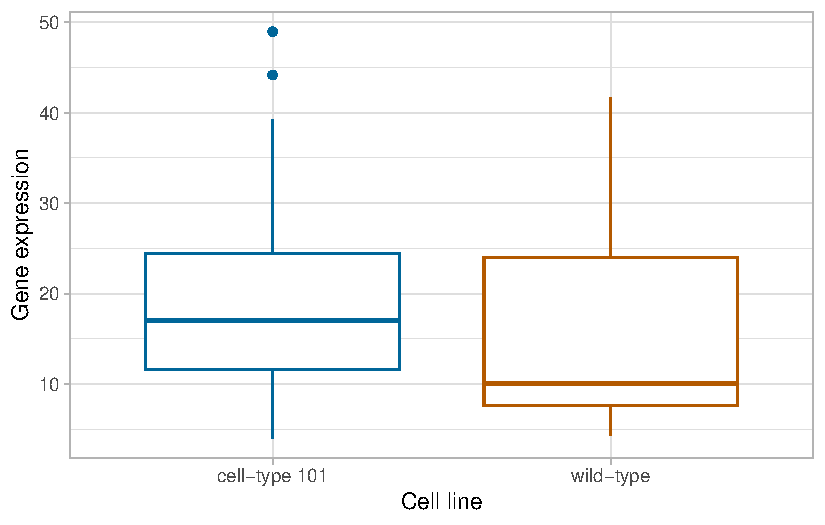
\includegraphics{2023-05-16_IMRaD-report_AStephenson_files/figure-pdf/fig-ge-cl-boxplot-1.pdf}

}

\caption{\label{fig-ge-cl-boxplot}A boxplot of gene expression for each
cell line (wild-type and cell-type 101).}

\end{figure}

A boxplot of gene expression, grouped by cell line, is shown in
Figure~\ref{fig-ge-cl-boxplot}. From this boxplot, it can be seen that
there does not appear to be a significant difference between gene
expression for wild-type and gene expression for cell-type 101. This
suggests that cell line may not be a predictor of gene expression, or at
least, not on its own.

\begin{figure}

{\centering 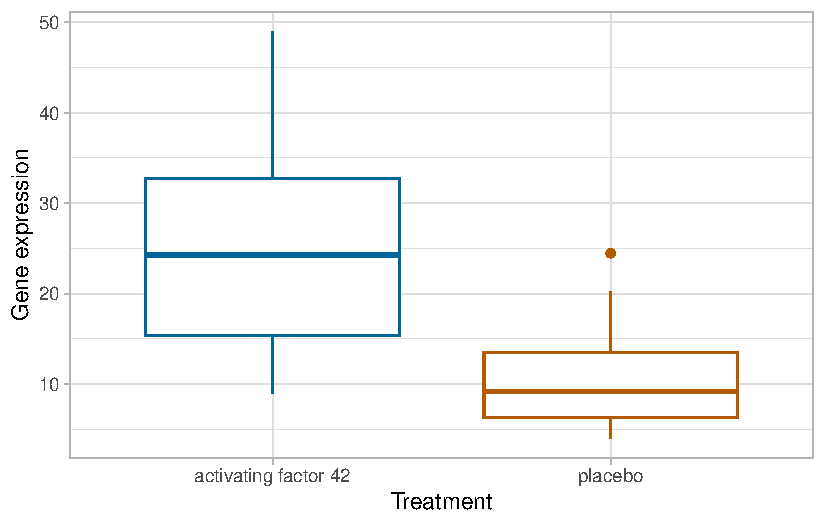
\includegraphics{2023-05-16_IMRaD-report_AStephenson_files/figure-pdf/fig-ge-treat-boxplot-1.pdf}

}

\caption{\label{fig-ge-treat-boxplot}A boxplot of gene expression for
each treatment (placebo and activating factor 42).}

\end{figure}

Figure~\ref{fig-ge-treat-boxplot} shows a boxplot of gene expression for
each treatment type (placebo or activating factor 42). From this
boxplot, it can be seen that there does appear to be a difference
between gene expression for placebo and gene expression for activating
factor 42. This suggests that treatment is a predictor of gene
expression.

\begin{figure}

{\centering 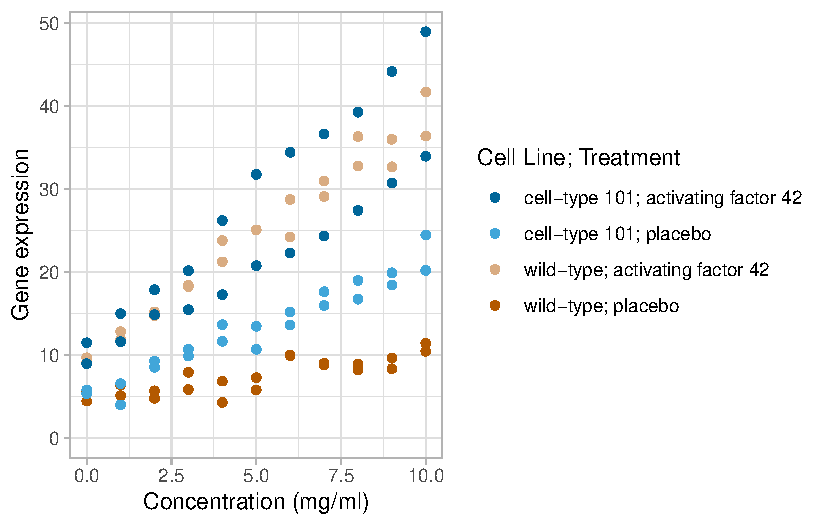
\includegraphics{2023-05-16_IMRaD-report_AStephenson_files/figure-pdf/fig-ge-conc-grouping-1.pdf}

}

\caption{\label{fig-ge-conc-grouping}A plot of gene expression as a
function of concentration, coloured by cell line (wild-type or cell-type
101) and treatment (placebo or activating factor 42).}

\end{figure}

The data is plotted in Figure~\ref{fig-ge-conc-grouping}, with gene
expression on the y axis and concentration on the x axis, with the data
points coloured by cell line and treatment. From this plot, it can be
seen that there does appear to be a relationship between concentration
and gene expression, which suggests that concentration is a predictor of
gene expression. From Figure~\ref{fig-ge-conc-grouping}, it can be seen
that there appear to be differences between the pairs (cell-type 101,
placebo) and (wild-type, placebo) and the other two pairs of cell line
and treatment. However, there does not appear to be a difference between
(cell-type 101, activating factor 42) and (wild-type, activating factor
42). This suggests that for the placebo treatment, cell line has an
impact on gene expression, but for the activating factor, cell line may
not have an impact on gene expression. Thus, cell line may be a
predictor for gene expression.

\textbf{REPEATED MEASURES HERE} Given that the gene expression for each
cell line and treatment was measured for different concentrations of
growth factor for the same gene line, then this must be taken into
account in fitting models on the data.

A linear model can be fit using the \texttt{step} function to select the
best model based on AIC, where the full scope is gene expression as a
function of concentration, treatment, and cell line, with interaction
terms between all three predictors. Using AIC, the function selects the
full model as the best model.

\begin{Shaded}
\begin{Highlighting}[]
\NormalTok{lm\_null \textless{}{-} lm(GE \textasciitilde{} 1, data = data\_long)}
\NormalTok{scope \textless{}{-} GE \textasciitilde{} concentration*treatment*CL}
\NormalTok{lm\_step \textless{}{-} step(lm\_null, scope = scope, direction = "both", trace = 0)}
\NormalTok{summary(lm\_step)}
\end{Highlighting}
\end{Shaded}

However, this does not consider the impact of gene line. A model can be
fitted for gene expression as a function of concentration, with gene
line as a random effect. The residuals plot for this model is shown in
Figure~\ref{fig-m1-plot}. From this figure, it can be seen that there is
still variance not explained by concentration alone, so this model will
not be considered further.

\begin{verbatim}
Linear mixed model fit by REML. t-tests use Satterthwaite's method [
lmerModLmerTest]
Formula: GE ~ concentration + (1 | GL)
   Data: data_long

REML criterion at convergence: 506.2

Scaled residuals: 
     Min       1Q   Median       3Q      Max 
-2.03686 -0.51171 -0.05062  0.55788  2.46633 

Random effects:
 Groups   Name        Variance Std.Dev.
 GL       (Intercept) 68.48    8.275   
 Residual             14.27    3.777   
Number of obs: 87, groups:  GL, 8

Fixed effects:
              Estimate Std. Error      df t value Pr(>|t|)    
(Intercept)     7.2948     3.0215  7.6657   2.414   0.0435 *  
concentration   2.0461     0.1273 78.0015  16.069   <2e-16 ***
---
Signif. codes:  0 '***' 0.001 '**' 0.01 '*' 0.05 '.' 0.1 ' ' 1

Correlation of Fixed Effects:
            (Intr)
concentratn -0.211
\end{verbatim}

\begin{figure}

{\centering 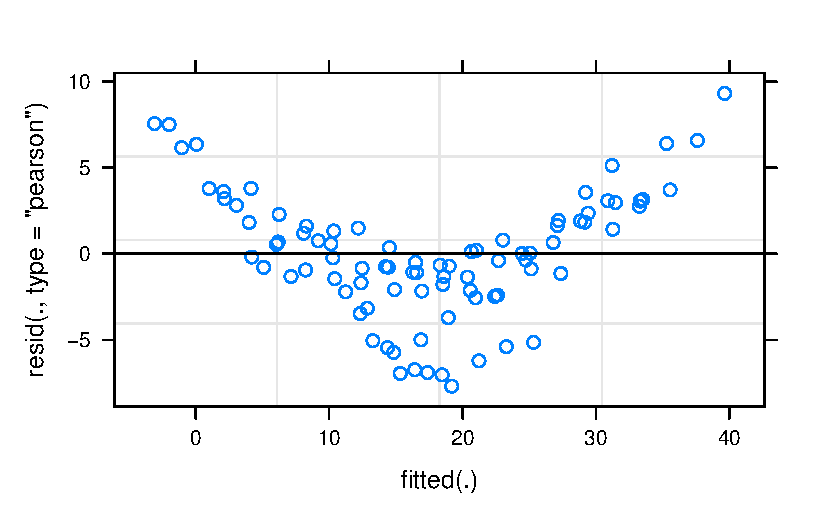
\includegraphics{2023-05-16_IMRaD-report_AStephenson_files/figure-pdf/fig-m1-plot-1.pdf}

}

\caption{\label{fig-m1-plot}The residuals plot for the model of gene
expression as a function of concentration, with gene line as a random
effect.}

\end{figure}

The next model considered fits gene expression as a function of
concentration and treatment (with interaction terms), as well as gene
line as a random effect. The residuals plot for this model is shown in
Figure~\ref{fig-m2-plot}.

\begin{verbatim}
Linear mixed model fit by REML. t-tests use Satterthwaite's method [
lmerModLmerTest]
Formula: GE ~ concentration * treatment + (1 | GL)
   Data: data_long

REML criterion at convergence: 396.5

Scaled residuals: 
     Min       1Q   Median       3Q      Max 
-1.84951 -0.73934 -0.04455  0.72880  2.38181 

Random effects:
 Groups   Name        Variance Std.Dev.
 GL       (Intercept) 12.609   3.551   
 Residual              4.255   2.063   
Number of obs: 87, groups:  GL, 8

Fixed effects:
                               Estimate Std. Error       df t value Pr(>|t|)
(Intercept)                     9.73729    1.86897  6.93144   5.210  0.00128
concentration                   2.99068    0.09834 77.00344  30.413  < 2e-16
treatmentplacebo               -4.88126    2.64267  6.92670  -1.847  0.10767
concentration:treatmentplacebo -1.88920    0.13907 77.00344 -13.585  < 2e-16
                                  
(Intercept)                    ** 
concentration                  ***
treatmentplacebo                  
concentration:treatmentplacebo ***
---
Signif. codes:  0 '***' 0.001 '**' 0.01 '*' 0.05 '.' 0.1 ' ' 1

Correlation of Fixed Effects:
            (Intr) cncntr trtmnt
concentratn -0.263              
tretmntplcb -0.707  0.186       
cncntrtn:tr  0.186 -0.707 -0.263
\end{verbatim}

\begin{figure}

{\centering 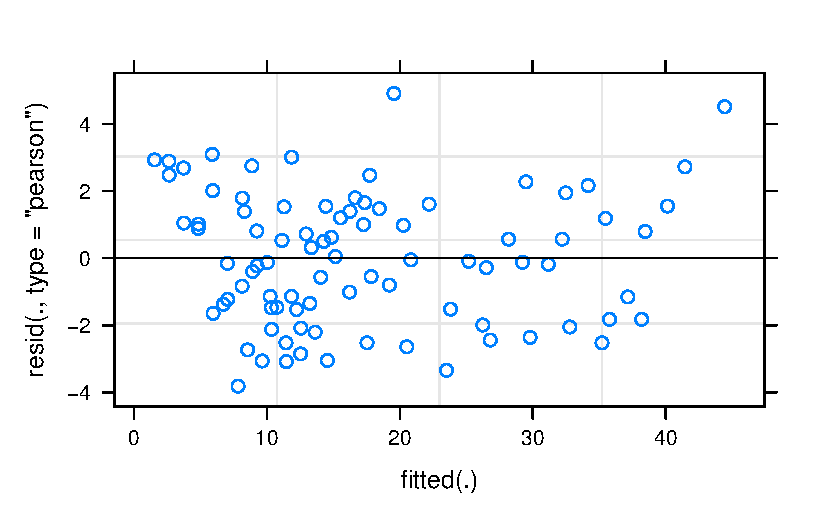
\includegraphics{2023-05-16_IMRaD-report_AStephenson_files/figure-pdf/fig-m2-plot-1.pdf}

}

\caption{\label{fig-m2-plot}The residuals plot for the model of gene
expression as a function of concentration and treatment (with
interaction terms), with gene line as a random effect.}

\end{figure}

Two models are fitted that include cell line as a predictor. One with
interaction terms between concentration and treatment only, and one with
interaction terms between concentration, treatment and cell line. The
residuals plots for these models are shown in Figure~\ref{fig-m3-plot}
and Figure~\ref{fig-m4-plot}, respectively.

\begin{verbatim}
Linear mixed model fit by REML. t-tests use Satterthwaite's method [
lmerModLmerTest]
Formula: GE ~ concentration * treatment + CL + (1 | GL)
   Data: data_long

REML criterion at convergence: 391

Scaled residuals: 
     Min       1Q   Median       3Q      Max 
-1.87305 -0.77007 -0.03212  0.71414  2.36286 

Random effects:
 Groups   Name        Variance Std.Dev.
 GL       (Intercept) 10.729   3.275   
 Residual              4.255   2.063   
Number of obs: 87, groups:  GL, 8

Fixed effects:
                               Estimate Std. Error       df t value Pr(>|t|)
(Intercept)                    11.40960    2.10015  5.59703   5.433  0.00201
concentration                   2.99068    0.09834 77.00431  30.413  < 2e-16
treatmentplacebo               -4.88000    2.45837  5.90950  -1.985  0.09509
CLwild-type                    -3.34716    2.35799  5.00431  -1.419  0.21493
concentration:treatmentplacebo -1.88920    0.13907 77.00431 -13.585  < 2e-16
                                  
(Intercept)                    ** 
concentration                  ***
treatmentplacebo               .  
CLwild-type                       
concentration:treatmentplacebo ***
---
Signif. codes:  0 '***' 0.001 '**' 0.01 '*' 0.05 '.' 0.1 ' ' 1

Correlation of Fixed Effects:
            (Intr) cncntr trtmnt CLwld-
concentratn -0.234                     
tretmntplcb -0.585  0.200              
CLwild-type -0.561  0.000  0.000       
cncntrtn:tr  0.166 -0.707 -0.283  0.000
\end{verbatim}

\begin{figure}

{\centering 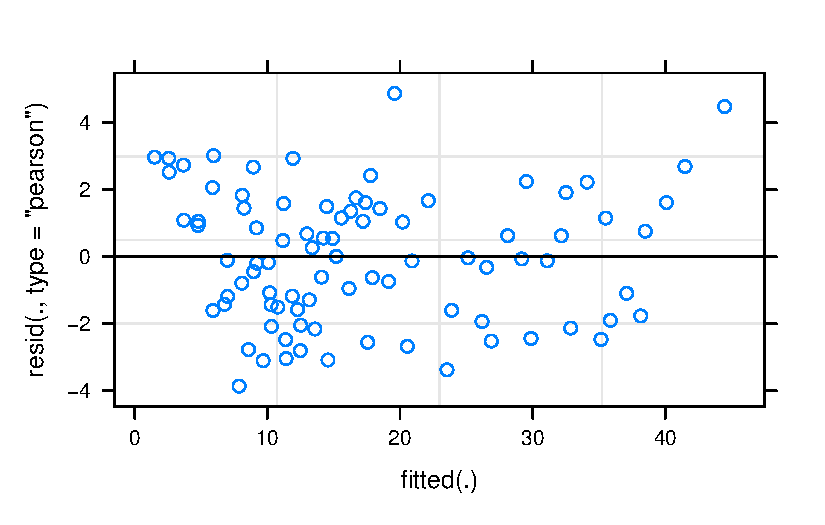
\includegraphics{2023-05-16_IMRaD-report_AStephenson_files/figure-pdf/fig-m3-plot-1.pdf}

}

\caption{\label{fig-m3-plot}The residuals plot for the model of gene
expression as a function of concentration and treatment (with
interaction terms) and cell line (without any interaction terms), with
gene line as a random effect.}

\end{figure}

\begin{verbatim}
Linear mixed model fit by REML. t-tests use Satterthwaite's method [
lmerModLmerTest]
Formula: GE ~ concentration * treatment * CL + (1 | GL)
   Data: data_long

REML criterion at convergence: 349.1

Scaled residuals: 
     Min       1Q   Median       3Q      Max 
-2.02535 -0.53265 -0.04358  0.58637  2.57581 

Random effects:
 Groups   Name        Variance Std.Dev.
 GL       (Intercept) 10.828   3.291   
 Residual              2.608   1.615   
Number of obs: 87, groups:  GL, 8

Fixed effects:
                                           Estimate Std. Error       df t value
(Intercept)                                 9.91750    2.41428  4.43886   4.108
concentration                               3.05141    0.10887 75.00175  28.027
treatmentplacebo                           -4.92159    3.41431  4.43886  -1.441
CLwild-type                                -0.36156    3.41518  4.44335  -0.106
concentration:treatmentplacebo             -1.40550    0.15397 75.00175  -9.128
concentration:CLwild-type                  -0.12145    0.15397 75.00175  -0.789
treatmentplacebo:CLwild-type                0.08179    4.82918  4.44111   0.017
concentration:treatmentplacebo:CLwild-type -0.96741    0.21775 75.00175  -4.443
                                           Pr(>|t|)    
(Intercept)                                  0.0119 *  
concentration                               < 2e-16 ***
treatmentplacebo                             0.2161    
CLwild-type                                  0.9203    
concentration:treatmentplacebo             8.48e-14 ***
concentration:CLwild-type                    0.4327    
treatmentplacebo:CLwild-type                 0.9872    
concentration:treatmentplacebo:CLwild-type 3.01e-05 ***
---
Signif. codes:  0 '***' 0.001 '**' 0.01 '*' 0.05 '.' 0.1 ' ' 1

Correlation of Fixed Effects:
            (Intr) cncntr trtmnt CLwld- cncnt: cn:CL- tr:CL-
concentratn -0.225                                          
tretmntplcb -0.707  0.159                                   
CLwild-type -0.707  0.159  0.500                            
cncntrtn:tr  0.159 -0.707 -0.225 -0.113                     
cncntrt:CL-  0.159 -0.707 -0.113 -0.225  0.500              
trtmntp:CL-  0.500 -0.113 -0.707 -0.707  0.159  0.159       
cncntr::CL- -0.113  0.500  0.159  0.159 -0.707 -0.707 -0.225
\end{verbatim}

\begin{figure}

{\centering 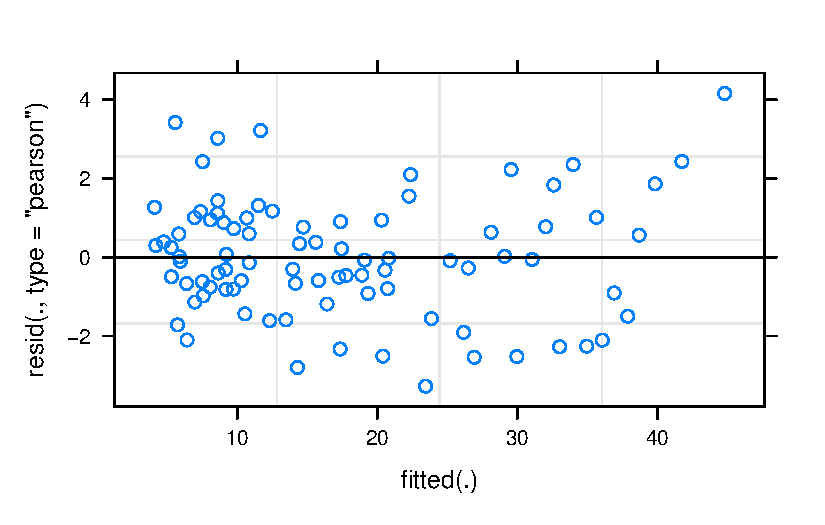
\includegraphics{2023-05-16_IMRaD-report_AStephenson_files/figure-pdf/fig-m4-plot-1.pdf}

}

\caption{\label{fig-m4-plot}The residuals plot for the model of gene
expression as a function of concentration, treatment and cell line (with
interaction terms between all three predictors), with gene line as a
random effect.}

\end{figure}

The residuals plots in Figure~\ref{fig-m2-plot} and
Figure~\ref{fig-m3-plot} both appear to not have any residual variance,
whilst the residuals plot for the model with interaction terms between
all three predictors (in Figure~\ref{fig-m4-plot}) appears to possibly
have some residual variance. \textbf{CHECK THIS}

\begin{table}

\caption{\textbf{?(caption)}}\begin{minipage}[t]{\linewidth}

{\centering 

~

}

\end{minipage}%
\newline
\begin{minipage}[t]{\linewidth}

{\centering 

GE

}

\end{minipage}%
\newline
\begin{minipage}[t]{\linewidth}

{\centering 

Predictors

}

\end{minipage}%
\newline
\begin{minipage}[t]{\linewidth}

{\centering 

Estimates

}

\end{minipage}%
\newline
\begin{minipage}[t]{\linewidth}

{\centering 

CI

}

\end{minipage}%
\newline
\begin{minipage}[t]{\linewidth}

{\centering 

p

}

\end{minipage}%
\newline
\begin{minipage}[t]{\linewidth}

{\centering 

(Intercept)

}

\end{minipage}%
\newline
\begin{minipage}[t]{\linewidth}

{\centering 

11.41

}

\end{minipage}%
\newline
\begin{minipage}[t]{\linewidth}

{\centering 

7.23~--~15.59

}

\end{minipage}%
\newline
\begin{minipage}[t]{\linewidth}

{\centering 

\textbf{\textless0.001}

}

\end{minipage}%
\newline
\begin{minipage}[t]{\linewidth}

{\centering 

concentration

}

\end{minipage}%
\newline
\begin{minipage}[t]{\linewidth}

{\centering 

2.99

}

\end{minipage}%
\newline
\begin{minipage}[t]{\linewidth}

{\centering 

2.79~--~3.19

}

\end{minipage}%
\newline
\begin{minipage}[t]{\linewidth}

{\centering 

\textbf{\textless0.001}

}

\end{minipage}%
\newline
\begin{minipage}[t]{\linewidth}

{\centering 

treatment {[}placebo{]}

}

\end{minipage}%
\newline
\begin{minipage}[t]{\linewidth}

{\centering 

-4.88

}

\end{minipage}%
\newline
\begin{minipage}[t]{\linewidth}

{\centering 

-9.77~--~0.01

}

\end{minipage}%
\newline
\begin{minipage}[t]{\linewidth}

{\centering 

0.051

}

\end{minipage}%
\newline
\begin{minipage}[t]{\linewidth}

{\centering 

CL {[}wild-type{]}

}

\end{minipage}%
\newline
\begin{minipage}[t]{\linewidth}

{\centering 

-3.35

}

\end{minipage}%
\newline
\begin{minipage}[t]{\linewidth}

{\centering 

-8.04~--~1.35

}

\end{minipage}%
\newline
\begin{minipage}[t]{\linewidth}

{\centering 

0.160

}

\end{minipage}%
\newline
\begin{minipage}[t]{\linewidth}

{\centering 

concentration * treatment\\
{[}placebo{]}

}

\end{minipage}%
\newline
\begin{minipage}[t]{\linewidth}

{\centering 

-1.89

}

\end{minipage}%
\newline
\begin{minipage}[t]{\linewidth}

{\centering 

-2.17~--~-1.61

}

\end{minipage}%
\newline
\begin{minipage}[t]{\linewidth}

{\centering 

\textbf{\textless0.001}

}

\end{minipage}%
\newline
\begin{minipage}[t]{\linewidth}

{\centering 

Random Effects

}

\end{minipage}%
\newline
\begin{minipage}[t]{\linewidth}

{\centering 

σ\textsuperscript{2}

}

\end{minipage}%
\newline
\begin{minipage}[t]{\linewidth}

{\centering 

4.25

}

\end{minipage}%
\newline
\begin{minipage}[t]{\linewidth}

{\centering 

τ\textsubscript{00} \textsubscript{GL}

}

\end{minipage}%
\newline
\begin{minipage}[t]{\linewidth}

{\centering 

10.73

}

\end{minipage}%
\newline
\begin{minipage}[t]{\linewidth}

{\centering 

ICC

}

\end{minipage}%
\newline
\begin{minipage}[t]{\linewidth}

{\centering 

0.72

}

\end{minipage}%
\newline
\begin{minipage}[t]{\linewidth}

{\centering 

N \textsubscript{GL}

}

\end{minipage}%
\newline
\begin{minipage}[t]{\linewidth}

{\centering 

8

}

\end{minipage}%
\newline
\begin{minipage}[t]{\linewidth}

{\centering 

Observations

}

\end{minipage}%
\newline
\begin{minipage}[t]{\linewidth}

{\centering 

87

}

\end{minipage}%
\newline
\begin{minipage}[t]{\linewidth}

{\centering 

Marginal R\textsuperscript{2} / Conditional R\textsuperscript{2}

}

\end{minipage}%
\newline
\begin{minipage}[t]{\linewidth}

{\centering 

0.877 / 0.965

}

\end{minipage}%

\end{table}

\textbf{?@tbl-sjPlot-m3} shows the estimates and p-values for these
estimates for the mixed effects model with concentration and treatment
(with the interaction term) and cell line (without interactions with
this predictor), as well as the gene line random effects. From this
table, it can be seen that the cell line predictor is not statistically
significant, so this term should be removed from the model. Removing
this term results in the mixed effects models with concentration and
treatment predictors (with the interaction term) and the gene line
random effects. The estimates for this model are shown in
\textbf{?@tbl-sjPlot-m2}, along with the p-values for these estimates.

\begin{table}

\caption{\textbf{?(caption)}}\begin{minipage}[t]{\linewidth}

{\centering 

~

}

\end{minipage}%
\newline
\begin{minipage}[t]{\linewidth}

{\centering 

GE

}

\end{minipage}%
\newline
\begin{minipage}[t]{\linewidth}

{\centering 

Predictors

}

\end{minipage}%
\newline
\begin{minipage}[t]{\linewidth}

{\centering 

Estimates

}

\end{minipage}%
\newline
\begin{minipage}[t]{\linewidth}

{\centering 

CI

}

\end{minipage}%
\newline
\begin{minipage}[t]{\linewidth}

{\centering 

p

}

\end{minipage}%
\newline
\begin{minipage}[t]{\linewidth}

{\centering 

(Intercept)

}

\end{minipage}%
\newline
\begin{minipage}[t]{\linewidth}

{\centering 

9.74

}

\end{minipage}%
\newline
\begin{minipage}[t]{\linewidth}

{\centering 

6.02~--~13.46

}

\end{minipage}%
\newline
\begin{minipage}[t]{\linewidth}

{\centering 

\textbf{\textless0.001}

}

\end{minipage}%
\newline
\begin{minipage}[t]{\linewidth}

{\centering 

concentration

}

\end{minipage}%
\newline
\begin{minipage}[t]{\linewidth}

{\centering 

2.99

}

\end{minipage}%
\newline
\begin{minipage}[t]{\linewidth}

{\centering 

2.80~--~3.19

}

\end{minipage}%
\newline
\begin{minipage}[t]{\linewidth}

{\centering 

\textbf{\textless0.001}

}

\end{minipage}%
\newline
\begin{minipage}[t]{\linewidth}

{\centering 

treatment {[}placebo{]}

}

\end{minipage}%
\newline
\begin{minipage}[t]{\linewidth}

{\centering 

-4.88

}

\end{minipage}%
\newline
\begin{minipage}[t]{\linewidth}

{\centering 

-10.14~--~0.38

}

\end{minipage}%
\newline
\begin{minipage}[t]{\linewidth}

{\centering 

0.068

}

\end{minipage}%
\newline
\begin{minipage}[t]{\linewidth}

{\centering 

concentration * treatment\\
{[}placebo{]}

}

\end{minipage}%
\newline
\begin{minipage}[t]{\linewidth}

{\centering 

-1.89

}

\end{minipage}%
\newline
\begin{minipage}[t]{\linewidth}

{\centering 

-2.17~--~-1.61

}

\end{minipage}%
\newline
\begin{minipage}[t]{\linewidth}

{\centering 

\textbf{\textless0.001}

}

\end{minipage}%
\newline
\begin{minipage}[t]{\linewidth}

{\centering 

Random Effects

}

\end{minipage}%
\newline
\begin{minipage}[t]{\linewidth}

{\centering 

σ\textsuperscript{2}

}

\end{minipage}%
\newline
\begin{minipage}[t]{\linewidth}

{\centering 

4.25

}

\end{minipage}%
\newline
\begin{minipage}[t]{\linewidth}

{\centering 

τ\textsubscript{00} \textsubscript{GL}

}

\end{minipage}%
\newline
\begin{minipage}[t]{\linewidth}

{\centering 

12.61

}

\end{minipage}%
\newline
\begin{minipage}[t]{\linewidth}

{\centering 

ICC

}

\end{minipage}%
\newline
\begin{minipage}[t]{\linewidth}

{\centering 

0.75

}

\end{minipage}%
\newline
\begin{minipage}[t]{\linewidth}

{\centering 

N \textsubscript{GL}

}

\end{minipage}%
\newline
\begin{minipage}[t]{\linewidth}

{\centering 

8

}

\end{minipage}%
\newline
\begin{minipage}[t]{\linewidth}

{\centering 

Observations

}

\end{minipage}%
\newline
\begin{minipage}[t]{\linewidth}

{\centering 

87

}

\end{minipage}%
\newline
\begin{minipage}[t]{\linewidth}

{\centering 

Marginal R\textsuperscript{2} / Conditional R\textsuperscript{2}

}

\end{minipage}%
\newline
\begin{minipage}[t]{\linewidth}

{\centering 

0.860 / 0.965

}

\end{minipage}%

\end{table}

\begin{table}

\caption{\textbf{?(caption)}}\begin{minipage}[t]{\linewidth}

{\centering 

~

}

\end{minipage}%
\newline
\begin{minipage}[t]{\linewidth}

{\centering 

GE

}

\end{minipage}%
\newline
\begin{minipage}[t]{\linewidth}

{\centering 

Predictors

}

\end{minipage}%
\newline
\begin{minipage}[t]{\linewidth}

{\centering 

Estimates

}

\end{minipage}%
\newline
\begin{minipage}[t]{\linewidth}

{\centering 

CI

}

\end{minipage}%
\newline
\begin{minipage}[t]{\linewidth}

{\centering 

p

}

\end{minipage}%
\newline
\begin{minipage}[t]{\linewidth}

{\centering 

(Intercept)

}

\end{minipage}%
\newline
\begin{minipage}[t]{\linewidth}

{\centering 

9.92

}

\end{minipage}%
\newline
\begin{minipage}[t]{\linewidth}

{\centering 

5.11~--~14.72

}

\end{minipage}%
\newline
\begin{minipage}[t]{\linewidth}

{\centering 

\textbf{\textless0.001}

}

\end{minipage}%
\newline
\begin{minipage}[t]{\linewidth}

{\centering 

concentration

}

\end{minipage}%
\newline
\begin{minipage}[t]{\linewidth}

{\centering 

3.05

}

\end{minipage}%
\newline
\begin{minipage}[t]{\linewidth}

{\centering 

2.83~--~3.27

}

\end{minipage}%
\newline
\begin{minipage}[t]{\linewidth}

{\centering 

\textbf{\textless0.001}

}

\end{minipage}%
\newline
\begin{minipage}[t]{\linewidth}

{\centering 

treatment {[}placebo{]}

}

\end{minipage}%
\newline
\begin{minipage}[t]{\linewidth}

{\centering 

-4.92

}

\end{minipage}%
\newline
\begin{minipage}[t]{\linewidth}

{\centering 

-11.72~--~1.88

}

\end{minipage}%
\newline
\begin{minipage}[t]{\linewidth}

{\centering 

0.154

}

\end{minipage}%
\newline
\begin{minipage}[t]{\linewidth}

{\centering 

CL {[}wild-type{]}

}

\end{minipage}%
\newline
\begin{minipage}[t]{\linewidth}

{\centering 

-0.36

}

\end{minipage}%
\newline
\begin{minipage}[t]{\linewidth}

{\centering 

-7.16~--~6.44

}

\end{minipage}%
\newline
\begin{minipage}[t]{\linewidth}

{\centering 

0.916

}

\end{minipage}%
\newline
\begin{minipage}[t]{\linewidth}

{\centering 

concentration * treatment\\
{[}placebo{]}

}

\end{minipage}%
\newline
\begin{minipage}[t]{\linewidth}

{\centering 

-1.41

}

\end{minipage}%
\newline
\begin{minipage}[t]{\linewidth}

{\centering 

-1.71~--~-1.10

}

\end{minipage}%
\newline
\begin{minipage}[t]{\linewidth}

{\centering 

\textbf{\textless0.001}

}

\end{minipage}%
\newline
\begin{minipage}[t]{\linewidth}

{\centering 

concentration * CL\\
{[}wild-type{]}

}

\end{minipage}%
\newline
\begin{minipage}[t]{\linewidth}

{\centering 

-0.12

}

\end{minipage}%
\newline
\begin{minipage}[t]{\linewidth}

{\centering 

-0.43~--~0.19

}

\end{minipage}%
\newline
\begin{minipage}[t]{\linewidth}

{\centering 

0.433

}

\end{minipage}%
\newline
\begin{minipage}[t]{\linewidth}

{\centering 

treatment {[}placebo{]} * CL\\
{[}wild-type{]}

}

\end{minipage}%
\newline
\begin{minipage}[t]{\linewidth}

{\centering 

0.08

}

\end{minipage}%
\newline
\begin{minipage}[t]{\linewidth}

{\centering 

-9.53~--~9.70

}

\end{minipage}%
\newline
\begin{minipage}[t]{\linewidth}

{\centering 

0.987

}

\end{minipage}%
\newline
\begin{minipage}[t]{\linewidth}

{\centering 

(concentration *\\
treatment {[}placebo{]}) * CL\\
{[}wild-type{]}

}

\end{minipage}%
\newline
\begin{minipage}[t]{\linewidth}

{\centering 

-0.97

}

\end{minipage}%
\newline
\begin{minipage}[t]{\linewidth}

{\centering 

-1.40~--~-0.53

}

\end{minipage}%
\newline
\begin{minipage}[t]{\linewidth}

{\centering 

\textbf{\textless0.001}

}

\end{minipage}%
\newline
\begin{minipage}[t]{\linewidth}

{\centering 

Random Effects

}

\end{minipage}%
\newline
\begin{minipage}[t]{\linewidth}

{\centering 

σ\textsuperscript{2}

}

\end{minipage}%
\newline
\begin{minipage}[t]{\linewidth}

{\centering 

2.61

}

\end{minipage}%
\newline
\begin{minipage}[t]{\linewidth}

{\centering 

τ\textsubscript{00} \textsubscript{GL}

}

\end{minipage}%
\newline
\begin{minipage}[t]{\linewidth}

{\centering 

10.83

}

\end{minipage}%
\newline
\begin{minipage}[t]{\linewidth}

{\centering 

ICC

}

\end{minipage}%
\newline
\begin{minipage}[t]{\linewidth}

{\centering 

0.81

}

\end{minipage}%
\newline
\begin{minipage}[t]{\linewidth}

{\centering 

N \textsubscript{GL}

}

\end{minipage}%
\newline
\begin{minipage}[t]{\linewidth}

{\centering 

8

}

\end{minipage}%
\newline
\begin{minipage}[t]{\linewidth}

{\centering 

Observations

}

\end{minipage}%
\newline
\begin{minipage}[t]{\linewidth}

{\centering 

87

}

\end{minipage}%
\newline
\begin{minipage}[t]{\linewidth}

{\centering 

Marginal R\textsuperscript{2} / Conditional R\textsuperscript{2}

}

\end{minipage}%
\newline
\begin{minipage}[t]{\linewidth}

{\centering 

0.891 / 0.979

}

\end{minipage}%

\end{table}

\textbf{?@tbl-sjPlot-m4} shows the estimates and p-values for the model
with concentration, treatment and cell line as predictors, along with
interaction terms between all predictors, and gene line random effects.
From this table, it can be seen that the interaction term between
concentration, treatment and cell line is statistically significant, so
this term should be kept. Because this term should be kept, then all of
the other fixed effect terms should also be kept.

\begin{table}

\caption{\textbf{?(caption)}}\begin{minipage}[t]{\linewidth}

{\centering 

~

}

\end{minipage}%
\newline
\begin{minipage}[t]{\linewidth}

{\centering 

GE

}

\end{minipage}%
\newline
\begin{minipage}[t]{\linewidth}

{\centering 

GE

}

\end{minipage}%
\newline
\begin{minipage}[t]{\linewidth}

{\centering 

GE

}

\end{minipage}%
\newline
\begin{minipage}[t]{\linewidth}

{\centering 

Predictors

}

\end{minipage}%
\newline
\begin{minipage}[t]{\linewidth}

{\centering 

Estimates

}

\end{minipage}%
\newline
\begin{minipage}[t]{\linewidth}

{\centering 

CI

}

\end{minipage}%
\newline
\begin{minipage}[t]{\linewidth}

{\centering 

p

}

\end{minipage}%
\newline
\begin{minipage}[t]{\linewidth}

{\centering 

Estimates

}

\end{minipage}%
\newline
\begin{minipage}[t]{\linewidth}

{\centering 

CI

}

\end{minipage}%
\newline
\begin{minipage}[t]{\linewidth}

{\centering 

p

}

\end{minipage}%
\newline
\begin{minipage}[t]{\linewidth}

{\centering 

Estimates

}

\end{minipage}%
\newline
\begin{minipage}[t]{\linewidth}

{\centering 

CI

}

\end{minipage}%
\newline
\begin{minipage}[t]{\linewidth}

{\centering 

p

}

\end{minipage}%
\newline
\begin{minipage}[t]{\linewidth}

{\centering 

(Intercept)

}

\end{minipage}%
\newline
\begin{minipage}[t]{\linewidth}

{\centering 

9.92

}

\end{minipage}%
\newline
\begin{minipage}[t]{\linewidth}

{\centering 

7.59~--~12.25

}

\end{minipage}%
\newline
\begin{minipage}[t]{\linewidth}

{\centering 

\textbf{\textless0.001}

}

\end{minipage}%
\newline
\begin{minipage}[t]{\linewidth}

{\centering 

9.74

}

\end{minipage}%
\newline
\begin{minipage}[t]{\linewidth}

{\centering 

6.02~--~13.46

}

\end{minipage}%
\newline
\begin{minipage}[t]{\linewidth}

{\centering 

\textbf{\textless0.001}

}

\end{minipage}%
\newline
\begin{minipage}[t]{\linewidth}

{\centering 

9.92

}

\end{minipage}%
\newline
\begin{minipage}[t]{\linewidth}

{\centering 

5.11~--~14.72

}

\end{minipage}%
\newline
\begin{minipage}[t]{\linewidth}

{\centering 

\textbf{\textless0.001}

}

\end{minipage}%
\newline
\begin{minipage}[t]{\linewidth}

{\centering 

concentration

}

\end{minipage}%
\newline
\begin{minipage}[t]{\linewidth}

{\centering 

3.05

}

\end{minipage}%
\newline
\begin{minipage}[t]{\linewidth}

{\centering 

2.66~--~3.45

}

\end{minipage}%
\newline
\begin{minipage}[t]{\linewidth}

{\centering 

\textbf{\textless0.001}

}

\end{minipage}%
\newline
\begin{minipage}[t]{\linewidth}

{\centering 

2.99

}

\end{minipage}%
\newline
\begin{minipage}[t]{\linewidth}

{\centering 

2.80~--~3.19

}

\end{minipage}%
\newline
\begin{minipage}[t]{\linewidth}

{\centering 

\textbf{\textless0.001}

}

\end{minipage}%
\newline
\begin{minipage}[t]{\linewidth}

{\centering 

3.05

}

\end{minipage}%
\newline
\begin{minipage}[t]{\linewidth}

{\centering 

2.83~--~3.27

}

\end{minipage}%
\newline
\begin{minipage}[t]{\linewidth}

{\centering 

\textbf{\textless0.001}

}

\end{minipage}%
\newline
\begin{minipage}[t]{\linewidth}

{\centering 

treatment {[}placebo{]}

}

\end{minipage}%
\newline
\begin{minipage}[t]{\linewidth}

{\centering 

-4.92

}

\end{minipage}%
\newline
\begin{minipage}[t]{\linewidth}

{\centering 

-8.22~--~-1.62

}

\end{minipage}%
\newline
\begin{minipage}[t]{\linewidth}

{\centering 

\textbf{0.004}

}

\end{minipage}%
\newline
\begin{minipage}[t]{\linewidth}

{\centering 

-4.88

}

\end{minipage}%
\newline
\begin{minipage}[t]{\linewidth}

{\centering 

-10.14~--~0.38

}

\end{minipage}%
\newline
\begin{minipage}[t]{\linewidth}

{\centering 

0.068

}

\end{minipage}%
\newline
\begin{minipage}[t]{\linewidth}

{\centering 

-4.92

}

\end{minipage}%
\newline
\begin{minipage}[t]{\linewidth}

{\centering 

-11.72~--~1.88

}

\end{minipage}%
\newline
\begin{minipage}[t]{\linewidth}

{\centering 

0.154

}

\end{minipage}%
\newline
\begin{minipage}[t]{\linewidth}

{\centering 

CL {[}wild-type{]}

}

\end{minipage}%
\newline
\begin{minipage}[t]{\linewidth}

{\centering 

-0.31

}

\end{minipage}%
\newline
\begin{minipage}[t]{\linewidth}

{\centering 

-3.62~--~2.99

}

\end{minipage}%
\newline
\begin{minipage}[t]{\linewidth}

{\centering 

0.850

}

\end{minipage}%
\newline
\begin{minipage}[t]{\linewidth}

{\centering 

-0.36

}

\end{minipage}%
\newline
\begin{minipage}[t]{\linewidth}

{\centering 

-7.16~--~6.44

}

\end{minipage}%
\newline
\begin{minipage}[t]{\linewidth}

{\centering 

0.916

}

\end{minipage}%
\newline
\begin{minipage}[t]{\linewidth}

{\centering 

concentration * treatment\\
{[}placebo{]}

}

\end{minipage}%
\newline
\begin{minipage}[t]{\linewidth}

{\centering 

-1.41

}

\end{minipage}%
\newline
\begin{minipage}[t]{\linewidth}

{\centering 

-1.96~--~-0.85

}

\end{minipage}%
\newline
\begin{minipage}[t]{\linewidth}

{\centering 

\textbf{\textless0.001}

}

\end{minipage}%
\newline
\begin{minipage}[t]{\linewidth}

{\centering 

-1.89

}

\end{minipage}%
\newline
\begin{minipage}[t]{\linewidth}

{\centering 

-2.17~--~-1.61

}

\end{minipage}%
\newline
\begin{minipage}[t]{\linewidth}

{\centering 

\textbf{\textless0.001}

}

\end{minipage}%
\newline
\begin{minipage}[t]{\linewidth}

{\centering 

-1.41

}

\end{minipage}%
\newline
\begin{minipage}[t]{\linewidth}

{\centering 

-1.71~--~-1.10

}

\end{minipage}%
\newline
\begin{minipage}[t]{\linewidth}

{\centering 

\textbf{\textless0.001}

}

\end{minipage}%
\newline
\begin{minipage}[t]{\linewidth}

{\centering 

concentration * CL\\
{[}wild-type{]}

}

\end{minipage}%
\newline
\begin{minipage}[t]{\linewidth}

{\centering 

-0.12

}

\end{minipage}%
\newline
\begin{minipage}[t]{\linewidth}

{\centering 

-0.68~--~0.44

}

\end{minipage}%
\newline
\begin{minipage}[t]{\linewidth}

{\centering 

0.666

}

\end{minipage}%
\newline
\begin{minipage}[t]{\linewidth}

{\centering 

-0.12

}

\end{minipage}%
\newline
\begin{minipage}[t]{\linewidth}

{\centering 

-0.43~--~0.19

}

\end{minipage}%
\newline
\begin{minipage}[t]{\linewidth}

{\centering 

0.433

}

\end{minipage}%
\newline
\begin{minipage}[t]{\linewidth}

{\centering 

treatment {[}placebo{]} * CL\\
{[}wild-type{]}

}

\end{minipage}%
\newline
\begin{minipage}[t]{\linewidth}

{\centering 

0.04

}

\end{minipage}%
\newline
\begin{minipage}[t]{\linewidth}

{\centering 

-4.64~--~4.71

}

\end{minipage}%
\newline
\begin{minipage}[t]{\linewidth}

{\centering 

0.988

}

\end{minipage}%
\newline
\begin{minipage}[t]{\linewidth}

{\centering 

0.08

}

\end{minipage}%
\newline
\begin{minipage}[t]{\linewidth}

{\centering 

-9.53~--~9.70

}

\end{minipage}%
\newline
\begin{minipage}[t]{\linewidth}

{\centering 

0.987

}

\end{minipage}%
\newline
\begin{minipage}[t]{\linewidth}

{\centering 

(concentration *\\
treatment {[}placebo{]}) * CL\\
{[}wild-type{]}

}

\end{minipage}%
\newline
\begin{minipage}[t]{\linewidth}

{\centering 

-0.97

}

\end{minipage}%
\newline
\begin{minipage}[t]{\linewidth}

{\centering 

-1.76~--~-0.18

}

\end{minipage}%
\newline
\begin{minipage}[t]{\linewidth}

{\centering 

\textbf{0.017}

}

\end{minipage}%
\newline
\begin{minipage}[t]{\linewidth}

{\centering 

-0.97

}

\end{minipage}%
\newline
\begin{minipage}[t]{\linewidth}

{\centering 

-1.40~--~-0.53

}

\end{minipage}%
\newline
\begin{minipage}[t]{\linewidth}

{\centering 

\textbf{\textless0.001}

}

\end{minipage}%
\newline
\begin{minipage}[t]{\linewidth}

{\centering 

Random Effects

}

\end{minipage}%
\newline
\begin{minipage}[t]{\linewidth}

{\centering 

σ\textsuperscript{2}

}

\end{minipage}%
\newline
\begin{minipage}[t]{\linewidth}

{\centering 

~

}

\end{minipage}%
\newline
\begin{minipage}[t]{\linewidth}

{\centering 

4.25

}

\end{minipage}%
\newline
\begin{minipage}[t]{\linewidth}

{\centering 

2.61

}

\end{minipage}%
\newline
\begin{minipage}[t]{\linewidth}

{\centering 

τ\textsubscript{00}

}

\end{minipage}%
\newline
\begin{minipage}[t]{\linewidth}

{\centering 

~

}

\end{minipage}%
\newline
\begin{minipage}[t]{\linewidth}

{\centering 

12.61 \textsubscript{GL}

}

\end{minipage}%
\newline
\begin{minipage}[t]{\linewidth}

{\centering 

10.83 \textsubscript{GL}

}

\end{minipage}%
\newline
\begin{minipage}[t]{\linewidth}

{\centering 

ICC

}

\end{minipage}%
\newline
\begin{minipage}[t]{\linewidth}

{\centering 

~

}

\end{minipage}%
\newline
\begin{minipage}[t]{\linewidth}

{\centering 

0.75

}

\end{minipage}%
\newline
\begin{minipage}[t]{\linewidth}

{\centering 

0.81

}

\end{minipage}%
\newline
\begin{minipage}[t]{\linewidth}

{\centering 

N

}

\end{minipage}%
\newline
\begin{minipage}[t]{\linewidth}

{\centering 

~

}

\end{minipage}%
\newline
\begin{minipage}[t]{\linewidth}

{\centering 

8 \textsubscript{GL}

}

\end{minipage}%
\newline
\begin{minipage}[t]{\linewidth}

{\centering 

8 \textsubscript{GL}

}

\end{minipage}%
\newline
\begin{minipage}[t]{\linewidth}

{\centering 

Observations

}

\end{minipage}%
\newline
\begin{minipage}[t]{\linewidth}

{\centering 

87

}

\end{minipage}%
\newline
\begin{minipage}[t]{\linewidth}

{\centering 

87

}

\end{minipage}%
\newline
\begin{minipage}[t]{\linewidth}

{\centering 

87

}

\end{minipage}%
\newline
\begin{minipage}[t]{\linewidth}

{\centering 

R\textsuperscript{2} / R\textsuperscript{2} adjusted

}

\end{minipage}%
\newline
\begin{minipage}[t]{\linewidth}

{\centering 

0.933 / 0.927

}

\end{minipage}%
\newline
\begin{minipage}[t]{\linewidth}

{\centering 

0.860 / 0.965

}

\end{minipage}%
\newline
\begin{minipage}[t]{\linewidth}

{\centering 

0.891 / 0.979

}

\end{minipage}%

\end{table}

The estimates for two remaining mixed effects models being studied are
shown in \textbf{?@tbl-sjPlot-step-m24}, along with fixed effects model.

\hypertarget{tbl-ranova-m2}{}
\begin{longtable}[]{@{}lrrrrrr@{}}
\caption{\label{tbl-ranova-m2}The results of the function
\texttt{ranova} applied to the mixed effects model with concentration
and treatment (and the interaction term between these predictors) as
fixed effects. \textbf{CHECK THIS}}\tabularnewline
\toprule()
& npar & logLik & AIC & LRT & Df & Pr(\textgreater Chisq) \\
\midrule()
\endfirsthead
\toprule()
& npar & logLik & AIC & LRT & Df & Pr(\textgreater Chisq) \\
\midrule()
\endhead
& 6 & -198.2331 & 408.4662 & & & \\
(1 \textbar{} GL) & 5 & -237.8918 & 485.7837 & 79.31749 & 1 &
5.288934e-19 \\
\bottomrule()
\end{longtable}

\hypertarget{tbl-ranova-m4}{}
\begin{longtable}[]{@{}lrrrrrr@{}}
\caption{\label{tbl-ranova-m4}The results of the function
\texttt{ranova} applied to the mixed effects model with concentration,
treatment and cell line (and the interaction terms between these
predictors) as fixed effects. \textbf{CHECK THIS}}\tabularnewline
\toprule()
& npar & logLik & AIC & LRT & Df & Pr(\textgreater Chisq) \\
\midrule()
\endfirsthead
\toprule()
& npar & logLik & AIC & LRT & Df & Pr(\textgreater Chisq) \\
\midrule()
\endhead
& 10 & -174.5644 & 369.1289 & & & \\
(1 \textbar{} GL) & 9 & -214.1471 & 446.2942 & 79.16527 & 1 &
5.712558e-19 \\
\bottomrule()
\end{longtable}

Table~\ref{tbl-ranova-m2} and Table~\ref{tbl-ranova-m4} show the results
of applying the function \texttt{ranova} to the two mixed effects models
considered. From these tables, it can be seen that the random effects
are significant in both models. Thus, these random effect terms should
not be removed.

\hypertarget{tbl-performance-m234}{}
\begin{longtable}[]{@{}lrrrr@{}}
\caption{\label{tbl-performance-m234}The AIC, R\(^{2}\) values and root
mean squared errors for each of the three fitted models.}\tabularnewline
\toprule()
Name & AIC & R2 & R2\_conditional & RMSE \\
\midrule()
\endfirsthead
\toprule()
Name & AIC & R2 & R2\_conditional & RMSE \\
\midrule()
\endhead
lm\_step & 443.9494 & 0.9327916 & & 2.798396 \\
m2 & 408.8027 & & 0.9647610 & 1.942813 \\
m4 & 372.5428 & & 0.9788391 & 1.500209 \\
\bottomrule()
\end{longtable}

The fixed effects model and mixed effects models can be compared to each
other using AIC values, R\(^{2}\) values and RMSE values (shown in
Table~\ref{tbl-performance-m234}). From these values, it can be seen
that the model with interaction terms between concentration, treatment
and cell line has the best AIC. The other two mixed effects models,
where there is either no interaction with cell line or cell line is not
a predictor, have very similar AIC values, whilst the model without
random effects has the worst AIC. The conditional R\(^{2}\) values,
which take into account both the fixed effects and the random effects,
are very similar for all models, but the model with all interaction
terms is still slightly better. The R\(^{2}\) value for the fixed
effects model is worse than the conditional R\(^{2}\) values for the
mixed effects models. The root mean square errors of the first two mixed
effects models in Table~\ref{tbl-performance-m234} are very similar,
whilst the root mean squared error for the fixed effects model is much
greater than the other values. The lowest root mean squared error occurs
for the mixed effects model with interaction terms between all three
predictors, suggesting that this model is the best. Thus, the model with
interaction terms between all three predictors, and with gene line as a
random effect, appears to be the best model.

\textbf{MORE HERE MAYBE}

\hypertarget{discussion}{%
\section{Discussion}\label{discussion}}

\textbf{TALK ABOUT CHOSEN MODEL AND HOW IT PREDICTS GENE EXPRESSION}

\begin{figure}

{\centering 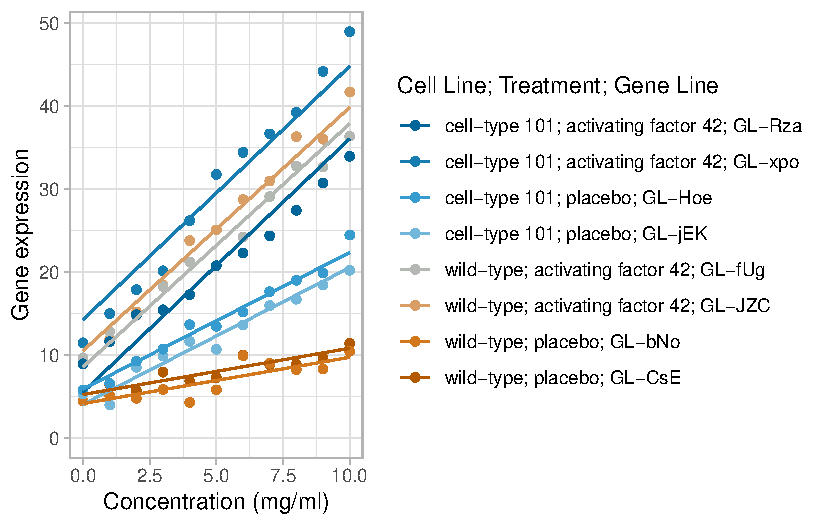
\includegraphics{2023-05-16_IMRaD-report_AStephenson_files/figure-pdf/fig-ge-conc-grouping-model-1.pdf}

}

\caption{\label{fig-ge-conc-grouping-model}A plot of gene expression as
a function of concentration, coloured by gene line (with cell line and
treatment also indicated), and with the fitted model indicated by the
lines.}

\end{figure}

The chosen model is the mixed effects model with concentration,
treatment and cell line as predictors, along with all interaction terms
between the three predictors, and gene line as a random effect. This
model is shown as the lines in Figure~\ref{fig-ge-conc-grouping-model},
where each line is the fitted model for a different gene line. This
figure shows how the gene lines with the placebo treatment (in darker
brown and lighter blue) have a flatter slope than the gene lines with
the activating factor 42 treatment (in lighter brown, grey and darker
blue). The slope of the fitted model for the wild-type cell lines with
the placebo treatments (in darker brown) is also flatter than the slope
of the fitted model for the cell-type 101 cell lines with the placebo
treatments (in lighter blue).

The coefficients of the fitted model are shown in
Table~\ref{tbl-fixed-coefs-m4}, and the random intercepts are shown in
Table~\ref{tbl-random-coefs-m4}. The intercept for each gene line is
found as the overall intercept (in Table~\ref{tbl-fixed-coefs-m4}) plus
the gene line specific intercept in Table~\ref{tbl-random-coefs-m4}.

\hypertarget{tbl-fixed-coefs-m4}{}
\begin{longtable}[]{@{}lr@{}}
\caption{\label{tbl-fixed-coefs-m4}The coefficients of the chosen model.
The value of the intercept is the overall intercept, which is added to
the values in Table~\ref{tbl-random-coefs-m4} to find the intercept for
each gene line. \textbf{CHECK THIS}}\tabularnewline
\toprule()
& value \\
\midrule()
\endfirsthead
\toprule()
& value \\
\midrule()
\endhead
(Intercept) & 9.9175000 \\
concentration & 3.0514091 \\
treatmentplacebo & -4.9215909 \\
CLwild-type & -0.3615634 \\
concentration:treatmentplacebo & -1.4055000 \\
concentration:CLwild-type & -0.1214545 \\
treatmentplacebo:CLwild-type & 0.0817907 \\
concentration:treatmentplacebo:CLwild-type & -0.9674091 \\
\bottomrule()
\end{longtable}

\hypertarget{tbl-random-coefs-m4}{}
\begin{longtable}[]{@{}lr@{}}
\caption{\label{tbl-random-coefs-m4}The difference from the overall
intercept for each gene line. \textbf{CHECK THIS}}\tabularnewline
\toprule()
& value \\
\midrule()
\endfirsthead
\toprule()
& value \\
\midrule()
\endhead
GL-bNo & -0.5448884 \\
GL-CsE & 0.5448884 \\
GL-fUg & -0.9801050 \\
GL-Hoe & 0.9171917 \\
GL-jEK & -0.9171917 \\
GL-JZC & 0.9801050 \\
GL-Rza & -4.3688926 \\
GL-xpo & 4.3688926 \\
\bottomrule()
\end{longtable}

From these tables, it can be seen that as growth factor concentration
increases, so does gene expression. It can also be seen that the placebo
treatment has a smaller intercept and flatter slope than the activating
factor 42 treatment does. Similarly, the wild-type cell line has a lower
intercept and flatter slope than the cell-type 101 cell line does. Thus,
gene expression is higher for higher concentrations of the growth
factor, the activating factor 42 treatment and cell-type 101 cell line.
Conversely, lower concentrations of the growth factor, the placebo
treatment and wild-type cell line results in lower gene expression.

\hypertarget{appendix-code}{%
\section{Appendix: Code}\label{appendix-code}}

\begin{Shaded}
\begin{Highlighting}[]
\NormalTok{pacman}\SpecialCharTok{::}\FunctionTok{p\_load}\NormalTok{(tidyverse, readr, lme4, knitr, performance, sjPlot, lmerTest)}
\FunctionTok{options}\NormalTok{(}\AttributeTok{knitr.kable.NA =} \StringTok{""}\NormalTok{)}
\FunctionTok{theme\_set}\NormalTok{(}\FunctionTok{theme\_light}\NormalTok{())}
\NormalTok{data }\OtherTok{\textless{}{-}} \FunctionTok{read\_csv}\NormalTok{(}\StringTok{"data/2023{-}03{-}01\_gene{-}data.csv"}\NormalTok{)}
\NormalTok{data\_long }\OtherTok{\textless{}{-}}\NormalTok{ data }\SpecialCharTok{\%\textgreater{}\%}
  \FunctionTok{mutate}\NormalTok{(}\AttributeTok{CL =} \StringTok{\textasciigrave{}}\AttributeTok{cell line}\StringTok{\textasciigrave{}}\NormalTok{,}
         \AttributeTok{treat =}\NormalTok{ treatment) }\SpecialCharTok{\%\textgreater{}\%}
  \FunctionTok{unite}\NormalTok{(}\StringTok{\textasciigrave{}}\AttributeTok{cell line}\StringTok{\textasciigrave{}}\NormalTok{, }\StringTok{\textasciigrave{}}\AttributeTok{treat}\StringTok{\textasciigrave{}}\NormalTok{, }\AttributeTok{sep =} \StringTok{"; "}\NormalTok{, }\AttributeTok{col =} \StringTok{"grouping"}\NormalTok{) }\SpecialCharTok{\%\textgreater{}\%}
  \FunctionTok{pivot\_longer}\NormalTok{(}\AttributeTok{cols =} \DecValTok{4}\SpecialCharTok{:}\DecValTok{14}\NormalTok{, }\AttributeTok{names\_to =} \StringTok{"concentration"}\NormalTok{, }\AttributeTok{values\_to =} \StringTok{"GE"}\NormalTok{) }\SpecialCharTok{\%\textgreater{}\%}
  \FunctionTok{filter}\NormalTok{(GE }\SpecialCharTok{\textgreater{}=} \DecValTok{0}\NormalTok{) }\SpecialCharTok{\%\textgreater{}\%}
  \FunctionTok{mutate}\NormalTok{(}\AttributeTok{concentration =} \FunctionTok{as.integer}\NormalTok{(concentration),}
         \AttributeTok{GL =} \FunctionTok{as.factor}\NormalTok{(sheet\_names),}
         \AttributeTok{CL =} \FunctionTok{as.factor}\NormalTok{(CL),}
         \AttributeTok{treatment =} \FunctionTok{as.factor}\NormalTok{(treatment),}
         \AttributeTok{grouping =} \FunctionTok{as.factor}\NormalTok{(grouping))}
\NormalTok{data\_long }\SpecialCharTok{\%\textgreater{}\%}
  \FunctionTok{ggplot}\NormalTok{(}\FunctionTok{aes}\NormalTok{(}\AttributeTok{x =}\NormalTok{ CL, }\AttributeTok{y =}\NormalTok{ GE, }\AttributeTok{col =}\NormalTok{ CL)) }\SpecialCharTok{+}
  \FunctionTok{geom\_boxplot}\NormalTok{() }\SpecialCharTok{+}
  \FunctionTok{theme}\NormalTok{(}\AttributeTok{legend.position =} \StringTok{\textquotesingle{}none\textquotesingle{}}\NormalTok{) }\SpecialCharTok{+}
\NormalTok{  harrypotter}\SpecialCharTok{::}\FunctionTok{scale\_color\_hp\_d}\NormalTok{(}\StringTok{"Ravenclaw"}\NormalTok{) }\SpecialCharTok{+}
  \FunctionTok{labs}\NormalTok{(}\AttributeTok{x =} \StringTok{"Cell line"}\NormalTok{,}
       \AttributeTok{y =} \StringTok{"Gene expression"}\NormalTok{)}
\NormalTok{data\_long }\SpecialCharTok{\%\textgreater{}\%}
  \FunctionTok{ggplot}\NormalTok{(}\FunctionTok{aes}\NormalTok{(}\AttributeTok{x =}\NormalTok{ treatment, }\AttributeTok{y =}\NormalTok{ GE, }\AttributeTok{col =}\NormalTok{ treatment)) }\SpecialCharTok{+}
  \FunctionTok{geom\_boxplot}\NormalTok{() }\SpecialCharTok{+}
  \FunctionTok{theme}\NormalTok{(}\AttributeTok{legend.position =} \StringTok{\textquotesingle{}none\textquotesingle{}}\NormalTok{) }\SpecialCharTok{+}
\NormalTok{  harrypotter}\SpecialCharTok{::}\FunctionTok{scale\_color\_hp\_d}\NormalTok{(}\StringTok{"Ravenclaw"}\NormalTok{) }\SpecialCharTok{+}
  \FunctionTok{labs}\NormalTok{(}\AttributeTok{x =} \StringTok{"Treatment"}\NormalTok{,}
       \AttributeTok{y =} \StringTok{"Gene expression"}\NormalTok{)}
\NormalTok{data\_long }\SpecialCharTok{\%\textgreater{}\%}
  \FunctionTok{ggplot}\NormalTok{(}\FunctionTok{aes}\NormalTok{(}\AttributeTok{x =}\NormalTok{ concentration, }\AttributeTok{y =}\NormalTok{ GE, }\AttributeTok{color =}\NormalTok{ grouping)) }\SpecialCharTok{+}
  \FunctionTok{geom\_point}\NormalTok{() }\SpecialCharTok{+}
  \FunctionTok{ylim}\NormalTok{(}\DecValTok{0}\NormalTok{, }\ConstantTok{NA}\NormalTok{) }\SpecialCharTok{+}
\NormalTok{  harrypotter}\SpecialCharTok{::}\FunctionTok{scale\_color\_hp\_d}\NormalTok{(}\StringTok{"Ravenclaw"}\NormalTok{) }\SpecialCharTok{+}
  \FunctionTok{labs}\NormalTok{(}\AttributeTok{x =} \StringTok{"Concentration (mg/ml)"}\NormalTok{,}
       \AttributeTok{y =} \StringTok{"Gene expression"}\NormalTok{,}
       \AttributeTok{color =} \StringTok{"Cell Line; Treatment"}\NormalTok{)}
\NormalTok{m1 }\OtherTok{\textless{}{-}} \FunctionTok{lmer}\NormalTok{(GE }\SpecialCharTok{\textasciitilde{}}\NormalTok{ concentration }\SpecialCharTok{+}\NormalTok{ (}\DecValTok{1}\SpecialCharTok{|}\NormalTok{GL), }\AttributeTok{data =}\NormalTok{ data\_long, }\AttributeTok{na.action =}\NormalTok{ na.omit)}
\FunctionTok{summary}\NormalTok{(m1)}
\FunctionTok{plot}\NormalTok{(m1)}
\NormalTok{m2 }\OtherTok{\textless{}{-}} \FunctionTok{lmer}\NormalTok{(GE }\SpecialCharTok{\textasciitilde{}}\NormalTok{ concentration}\SpecialCharTok{*}\NormalTok{treatment }\SpecialCharTok{+}\NormalTok{ (}\DecValTok{1}\SpecialCharTok{|}\NormalTok{GL), }\AttributeTok{data =}\NormalTok{ data\_long, }\AttributeTok{na.action =}\NormalTok{ na.omit)}
\FunctionTok{summary}\NormalTok{(m2)}
\FunctionTok{plot}\NormalTok{(m2)}
\NormalTok{m3 }\OtherTok{\textless{}{-}} \FunctionTok{lmer}\NormalTok{(GE }\SpecialCharTok{\textasciitilde{}}\NormalTok{ concentration}\SpecialCharTok{*}\NormalTok{treatment }\SpecialCharTok{+}\NormalTok{ CL }\SpecialCharTok{+}\NormalTok{ (}\DecValTok{1}\SpecialCharTok{|}\NormalTok{GL), }\AttributeTok{data =}\NormalTok{ data\_long, }\AttributeTok{na.action =}\NormalTok{ na.omit)}
\FunctionTok{summary}\NormalTok{(m3)}
\FunctionTok{plot}\NormalTok{(m3)}
\NormalTok{m4 }\OtherTok{\textless{}{-}} \FunctionTok{lmer}\NormalTok{(GE }\SpecialCharTok{\textasciitilde{}}\NormalTok{ concentration}\SpecialCharTok{*}\NormalTok{treatment}\SpecialCharTok{*}\NormalTok{CL }\SpecialCharTok{+}\NormalTok{ (}\DecValTok{1}\SpecialCharTok{|}\NormalTok{GL), }\AttributeTok{data =}\NormalTok{ data\_long, }\AttributeTok{na.action =}\NormalTok{ na.omit)}
\FunctionTok{summary}\NormalTok{(m4)}
\FunctionTok{plot}\NormalTok{(m4)}
\FunctionTok{tab\_model}\NormalTok{(m3)}
\FunctionTok{tab\_model}\NormalTok{(m2)}
\FunctionTok{tab\_model}\NormalTok{(m4)}
\NormalTok{lm\_step }\OtherTok{\textless{}{-}} \FunctionTok{lm}\NormalTok{(GE }\SpecialCharTok{\textasciitilde{}}\NormalTok{ concentration}\SpecialCharTok{*}\NormalTok{treatment}\SpecialCharTok{*}\NormalTok{CL, }\AttributeTok{data =}\NormalTok{ data\_long)}
\FunctionTok{tab\_model}\NormalTok{(lm\_step, m2, m4)}
\FunctionTok{ranova}\NormalTok{(m2) }\SpecialCharTok{\%\textgreater{}\%} 
  \FunctionTok{kable}\NormalTok{(}\AttributeTok{digits =} \FunctionTok{c}\NormalTok{(}\DecValTok{0}\NormalTok{,}\DecValTok{4}\NormalTok{,}\DecValTok{4}\NormalTok{,}\DecValTok{5}\NormalTok{,}\DecValTok{4}\NormalTok{,}\DecValTok{25}\NormalTok{))}
\FunctionTok{ranova}\NormalTok{(m4) }\SpecialCharTok{\%\textgreater{}\%} 
  \FunctionTok{kable}\NormalTok{(}\AttributeTok{digits =} \FunctionTok{c}\NormalTok{(}\DecValTok{0}\NormalTok{,}\DecValTok{4}\NormalTok{,}\DecValTok{4}\NormalTok{,}\DecValTok{5}\NormalTok{,}\DecValTok{4}\NormalTok{,}\DecValTok{25}\NormalTok{))}
\FunctionTok{compare\_performance}\NormalTok{(lm\_step, m2, m4) }\SpecialCharTok{\%\textgreater{}\%} 
  \FunctionTok{select}\NormalTok{(}\FunctionTok{c}\NormalTok{(}\StringTok{"Name"}\NormalTok{, }\StringTok{"AIC"}\NormalTok{, }\StringTok{"R2"}\NormalTok{, }\StringTok{"R2\_conditional"}\NormalTok{, }\StringTok{"RMSE"}\NormalTok{)) }\SpecialCharTok{\%\textgreater{}\%} 
  \FunctionTok{kable}\NormalTok{(}\AttributeTok{digits =} \FunctionTok{c}\NormalTok{(}\DecValTok{0}\NormalTok{,}\DecValTok{4}\NormalTok{,}\DecValTok{7}\NormalTok{,}\DecValTok{7}\NormalTok{,}\DecValTok{6}\NormalTok{))}
\NormalTok{data\_long }\SpecialCharTok{\%\textgreater{}\%}
  \FunctionTok{mutate}\NormalTok{(}\AttributeTok{group =}\NormalTok{ grouping,}
         \AttributeTok{geneline =}\NormalTok{ GL) }\SpecialCharTok{\%\textgreater{}\%}
  \FunctionTok{unite}\NormalTok{(group, geneline, }\AttributeTok{sep =} \StringTok{"; "}\NormalTok{, }\AttributeTok{col =} \StringTok{"grouping2"}\NormalTok{) }\SpecialCharTok{\%\textgreater{}\%}
  \FunctionTok{ggplot}\NormalTok{(}\FunctionTok{aes}\NormalTok{(}\AttributeTok{x =}\NormalTok{ concentration, }\AttributeTok{y =}\NormalTok{ GE, }\AttributeTok{color =}\NormalTok{ grouping2)) }\SpecialCharTok{+}
  \FunctionTok{geom\_point}\NormalTok{() }\SpecialCharTok{+}
  \FunctionTok{geom\_line}\NormalTok{(}\FunctionTok{aes}\NormalTok{(}\AttributeTok{y =} \FunctionTok{predict}\NormalTok{(m4))) }\SpecialCharTok{+}
  \FunctionTok{ylim}\NormalTok{(}\DecValTok{0}\NormalTok{, }\ConstantTok{NA}\NormalTok{) }\SpecialCharTok{+}
  \CommentTok{\# scale\_color\_manual(values=c("\#006699", "\#006699", "\#98C2D9", "\#98C2D9", "\#D9AC82", "\#D9AC82", "\#B35900", "\#B35900")) +}
\NormalTok{  harrypotter}\SpecialCharTok{::}\FunctionTok{scale\_color\_hp\_d}\NormalTok{(}\StringTok{"Ravenclaw"}\NormalTok{) }\SpecialCharTok{+}
  \FunctionTok{labs}\NormalTok{(}\AttributeTok{x =} \StringTok{"Concentration (mg/ml)"}\NormalTok{,}
       \AttributeTok{y =} \StringTok{"Gene expression"}\NormalTok{,}
       \AttributeTok{color =} \StringTok{"Cell Line; Treatment; Gene Line"}\NormalTok{)}
\FunctionTok{fixef}\NormalTok{(m4) }\SpecialCharTok{\%\textgreater{}\%} 
  \FunctionTok{data.frame}\NormalTok{() }\SpecialCharTok{\%\textgreater{}\%} 
  \FunctionTok{rename}\NormalTok{(}\AttributeTok{value =} \StringTok{"."}\NormalTok{) }\SpecialCharTok{\%\textgreater{}\%}
  \FunctionTok{kable}\NormalTok{()}
\NormalTok{random\_effects }\OtherTok{\textless{}{-}} \FunctionTok{ranef}\NormalTok{(m4)}\SpecialCharTok{$}\NormalTok{GL}
\NormalTok{random\_effects }\SpecialCharTok{\%\textgreater{}\%}
  \FunctionTok{rename}\NormalTok{(}\AttributeTok{value =} \StringTok{\textasciigrave{}}\AttributeTok{(Intercept)}\StringTok{\textasciigrave{}}\NormalTok{) }\SpecialCharTok{\%\textgreater{}\%} 
  \FunctionTok{kable}\NormalTok{()}
\end{Highlighting}
\end{Shaded}

\hypertarget{refs}{}
\begin{CSLReferences}{1}{0}
\leavevmode\vadjust pre{\hypertarget{ref-lme4}{}}%
Bates, Douglas, Martin Mächler, Ben Bolker, and Steve Walker. 2015.
{``Fitting Linear Mixed-Effects Models Using {lme4}.''} \emph{Journal of
Statistical Software} 67 (1): 1--48.
\url{https://doi.org/10.18637/jss.v067.i01}.

\leavevmode\vadjust pre{\hypertarget{ref-ggpubr}{}}%
Kassambara, Alboukadel. 2023a. \emph{{ggpubr}: '{ggplot2}' Based
Publication Ready Plots}.
\url{https://CRAN.R-project.org/package=ggpubr}.

\leavevmode\vadjust pre{\hypertarget{ref-rstatix}{}}%
---------. 2023b. \emph{{rstatix}: Pipe-Friendly Framework for Basic
Statistical Tests}. \url{https://CRAN.R-project.org/package=rstatix}.

\leavevmode\vadjust pre{\hypertarget{ref-lmerTest}{}}%
Kuznetsova, Alexandra, Per B. Brockhoff, and Rune H. B. Christensen.
2017. {``{lmerTest} Package: Tests in Linear Mixed Effects Models.''}
\emph{Journal of Statistical Software} 82 (13): 1--26.
\url{https://doi.org/10.18637/jss.v082.i13}.

\leavevmode\vadjust pre{\hypertarget{ref-sjPlot}{}}%
Lüdecke, Daniel. 2023. \emph{{sjPlot}: Data Visualization for Statistics
in Social Science}. \url{https://CRAN.R-project.org/package=sjPlot}.

\leavevmode\vadjust pre{\hypertarget{ref-performance}{}}%
Lüdecke, Daniel, Mattan S. Ben-Shachar, Indrajeet Patil, Philip
Waggoner, and Dominique Makowski. 2021. {``{performance}: An {R} Package
for Assessment, Comparison and Testing of Statistical Models.''}
\emph{Journal of Open Source Software} 6 (60): 3139.
\url{https://doi.org/10.21105/joss.03139}.

\leavevmode\vadjust pre{\hypertarget{ref-patchwork}{}}%
Pedersen, Thomas Lin. 2022. \emph{{patchwork}: The Composer of Plots}.
\url{https://CRAN.R-project.org/package=patchwork}.

\leavevmode\vadjust pre{\hypertarget{ref-showtext}{}}%
Qiu, Yixuan, and authors/contributors of the included software. 2022.
\emph{{showtext}: Using Fonts More Easily in r Graphs}.
\url{https://CRAN.R-project.org/package=showtext}.

\leavevmode\vadjust pre{\hypertarget{ref-r-2022}{}}%
R Core Team. 2022. \emph{R: A Language and Environment for Statistical
Computing}. Vienna, Austria: R Foundation for Statistical Computing.
\url{https://www.R-project.org/}.

\leavevmode\vadjust pre{\hypertarget{ref-ggrepel}{}}%
Slowikowski, Kamil. 2023. \emph{{ggrepel}: Automatically Position
Non-Overlapping Text Labels with '{ggplot2}'}.
\url{https://CRAN.R-project.org/package=ggrepel}.

\leavevmode\vadjust pre{\hypertarget{ref-tidyverse}{}}%
Wickham, Hadley, Mara Averick, Jennifer Bryan, Winston Chang, Lucy
D'Agostino McGowan, Romain François, Garrett Grolemund, et al. 2019.
{``Welcome to the {tidyverse}.''} \emph{Journal of Open Source Software}
4 (43): 1686. \url{https://doi.org/10.21105/joss.01686}.

\leavevmode\vadjust pre{\hypertarget{ref-readr}{}}%
Wickham, Hadley, Jim Hester, and Jennifer Bryan. 2023. \emph{{readr}:
Read Rectangular Text Data}.
\url{https://CRAN.R-project.org/package=readr}.

\leavevmode\vadjust pre{\hypertarget{ref-knitr}{}}%
Xie, Yihui. 2023. \emph{{knitr}: A General-Purpose Package for Dynamic
Report Generation in r}. \url{https://yihui.org/knitr/}.

\end{CSLReferences}



\end{document}
